\chapter*{Appendix}
\subsection*{Différentes requêtes}
\subsubsection*{Pour les Galaxies}
\noindent SELECT TOP 200000\\
p.objid, s.rowc\_u, s.rowc\_i, s.rowc\_z, s.rowc\_g, s.rowc\_r, s.colc\_u, s.colc\_i, s.colc\_z,s.colc\_g, s.colc\_r, p.rerun, p.run, p.camcol, p.field, p.z as redshift, p.class \\
FROM SpecPhoto AS p JOIN PhotoPrimary AS s ON s.objid = p.objid\\
where p.class = 'GALAXIES'
\subsubsection*{Pour les Quazars}
\noindent SELECT TOP 200000\\
p.objid, s.rowc\_u, s.rowc\_i, s.rowc\_z, s.rowc\_g, s.rowc\_r, s.colc\_u, s.colc\_i, s.colc\_z, s.colc\_g, s.colc\_r, p.rerun, p.run, p.camcol, p.field, p.z as redshift,p.class \\
FROM SpecPhoto AS p JOIN PhotoPrimary AS s ON s.objid = p.objid\\
where p.class = 'QSO'
\subsubsection*{Pour les étoiles}
\noindent SELECT TOP 200000\\
p.objid, s.rowc\_u, s.rowc\_i, s.rowc\_z, s.rowc\_g, s.rowc\_r, s.colc\_u, s.colc\_i, s.colc\_z, s.colc\_g, s.colc\_r, p.rerun, p.run, p.camcol, p.field, p.z as redshift, p.class\\
FROM SpecPhoto AS p JOIN PhotoPrimary AS s ON s.objid = p.objid\\
where p.class = 'STAR'
\subsubsection*{Codes}
\textit{https://github.com/oussissa123/redshift\_estimation}
\subsection*{Quelques figures}

\begin{figure}[H]
	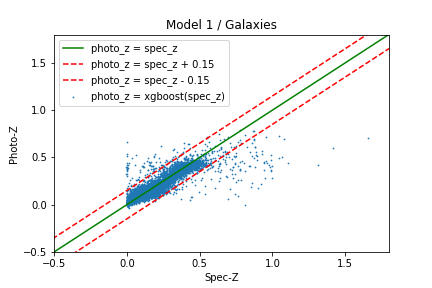
\includegraphics[scale = 0.4]{images/model1_galaxies.png}
	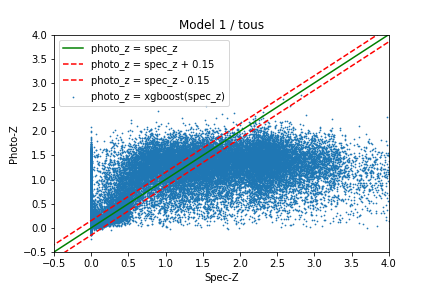
\includegraphics[scale = 0.4]{images/model1_tous.png}
	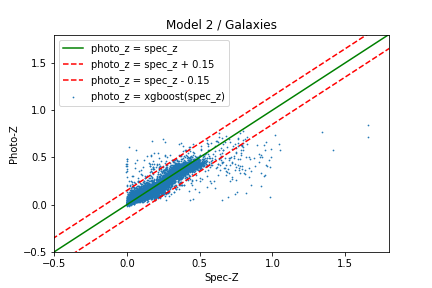
\includegraphics[scale = 0.4]{images/model2_galaxies.png}
	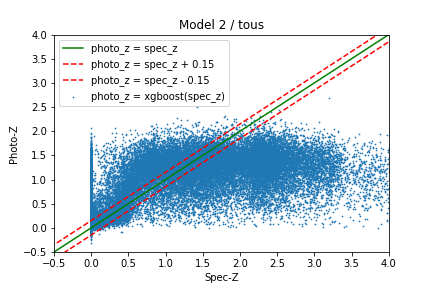
\includegraphics[scale = 0.4]{images/model2_tous.png}
	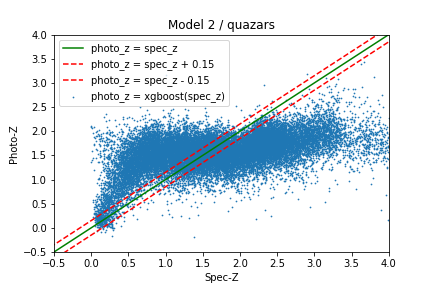
\includegraphics[scale = 0.4]{images/model2_quazars.png}
	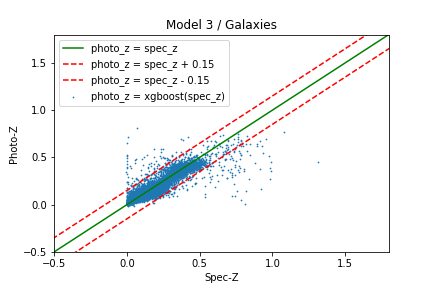
\includegraphics[scale = 0.4]{images/model3_galaxies.png}
	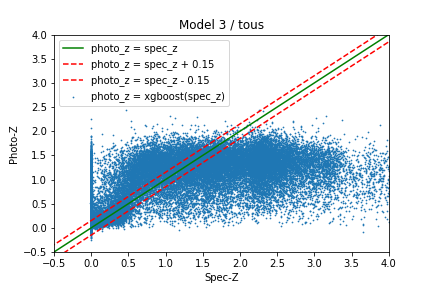
\includegraphics[scale = 0.4]{images/model3_tous.png}
	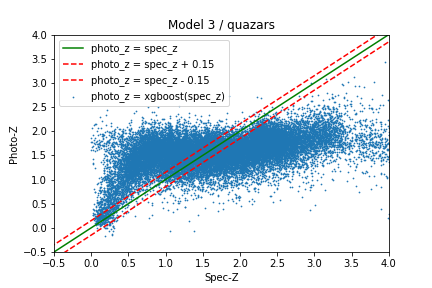
\includegraphics[scale = 0.4]{images/model3_quazars.png}
	\caption{Perturbation entre les valeurs spectroscopiques et photométriques à partir du modèle Boosting sur l'ensemble de test}
\end{figure}
